\chapter{Tervez\'es}\label{chapter:tervezes}
Ebben a fejezetben a "WatchWithFriends" alkalmazás tervezési folyamatát mutatom be.
A fejezet első részében a felhasználói felület tervezését ismertetem,
majd a szerver és a kliens közötti kommunikáció megvalósítását.

\section*{Felhasználói felület tervezése}
FELHASZNÁLÓI FELÜLET!!!


\section*{Szerver oldali logika megtervezése}
\subsection*{Architektúra}
Az alkalmazásnál MVC (Model-View-Controller) architektúrára építettem, illetve
bővítettem a Repository és a Service rétegekkel. Az MVC architektúra egy
architektúrális minta, amely a felhasználói felületet (View), az alkalmazás
logikáját (Controller) és az adatokat (Model) három különálló részre osztja.
A Repository réteg a Model réteghez tartozik, a Service réteg pedig a Controller réteghez.
Azért bontottam tovább a rétegeket, mert így jobban elkülönülnek a felelősségi körök,
és a kód is átláthatóbb lesz, illetve könnyebben bővíthető, és tesztelhető lesz.
\\
\\
\begin{figure}[H]
    \centering
    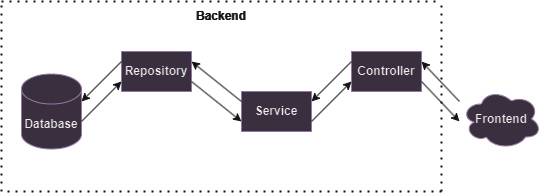
\includegraphics[width=14.0truecm]{images/BackendArchitecture.png}
    \caption{Backend Architektúra}
    \label{fig:backend_architecture}
\end{figure}
\textbf{Ismertetem a rétegek főbb tulajdonságait:}
\begin{itemize}
    \item \textbf{Adatbázis}: Az alkalmazásom adattára. Itt tárolódnak a statikus és dinamikus adatok.
    \item \textbf{Repositoryk}: Az adatbázis és az alkalmazás logikája közötti köztes réteg. CRUD műveletek, komplex lekérdezések.
    \item \textbf{Servicek}: Az üzleti logika helye. Itt történnek a komplex számítások, validációk és egyéb logikai műveletek.
    \item \textbf{Controllerek}: Az API végpontokat kezelő réteg. Fogadják a kliens kéréseit, és válaszokat generálnak.
\end{itemize}

\subsection*{Szoftvertervezési elvek (tervezés)}
A szoftvertervezési elvek alapvető útmutatások a kiváló kód fejlesztéséhez. Ezek az iránymutatások növelik a kód minőségét, gyorsítják a fejlesztési folyamatot és minimalizálják a hibalehetőségeket. Az ilyen elvek segítenek abban, hogy a kód könnyen újrafelhasználható és karbantartható legyen.

A kód olvashatóságát és tesztelhetőségét is javítják, ami hosszú távon időt és erőforrást spórol. A rugalmasság és a bővíthetőség is nő, tehát a kód könnyen adaptálható új funkciók vagy változások esetén. Továbbá, ezek az elvek arra is ösztönöznek, hogy egyszerű és nem redundáns kódot írj, ami csökkenti a komplexitást és növeli a kohéziót. Az elvek célja a kód moduláris felépítése és az alacsonyabb összekapcsoltság, ami hozzájárul a jobb szervezettséghez és könnyebb karbantartáshoz.

Összességében, a szoftvertervezési elvek olyan iránymutatások, amelyek célja a hatékony, karbantartható és minőségi kód létrehozása.
Én a SOLID elveket használtam a szoftvertervezési elvek közül, mert ezeket a leggyakrabban használják, és a legtöbb fejlesztő ismeri őket.
\\
\\
\textbf{Ismertetem a SOLID elvek főbb tulajdonságait:}
\begin{itemize}
    \item \textbf{Single Responsibility Principle (SRP)}: Egy osztály vagy modul csak egy felelősséggel rendelkezzen.
    \item \textbf{Open-Closed Principle (OCP)}: Nyitva áll, de nem módosítható. A kód legyen könnyen bővíthető, de ne kelljen módosítani a meglévő kódot.
    \item \textbf{Liskov Substitution Principle (LSP)}: A leszármazott osztályok legyenek helyettesíthetők az ősosztályokkal.
    \item \textbf{Interface Segregation Principle (ISP)}: A kliensek ne függjenek olyan interfészektől, amelyeket nem használnak.
    \item \textbf{Dependency Inversion Principle (DIP)}: A függőségek irányát fordítsuk meg, és a magasabb szintű modulok ne függjenek a részletektől.
\end{itemize}
